%!TEX TS-program = xelatex
\documentclass[]{shiltemann-cv}
\addbibresource{publications.bib}
\usepackage{fontspec}
\defaultfontfeatures{Path = /usr/share/texlive/texmf-dist/fonts/opentype/public/fontawesome/}
\usepackage{fontawesome}

\begin{document}
\header{Saskia}{Hiltemann}
       {Post-Doctoral Researcher, Bioinformatics \& Education}


% In the aside, each new line forces a line break
\begin{aside}
  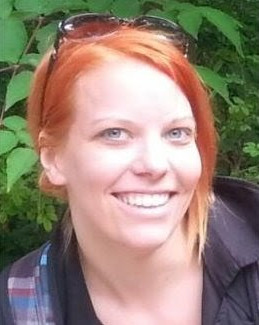
\includegraphics[width=75pt]{foto.jpg}
  \section{About}
    De Carpentierstraat 24
    2595HL, Den Haag
    The Netherlands
    ~
    saskiahilltemann @gmail.com \faEnvelope
    shiltemann \faGithub \ \faTwitter \ \faLinkedin
    \
    \ \\
    ORCID:
    0000-0003-3803-468X \faOrcid
  \section{Languages}
    Bilingual Dutch/English
    German \& French
  \section{Skills}
    Python, C, C++, UNIX, Galaxy, Docker, Jekyll, LaTeX
\end{aside}

\section{Interests}

Bioinformatics, Education \& Training, Open Science, FAIR principles, Community Building, Genome Sequencing, Data Analysis, Workflows, Automation, Visualisation, Best Practices, Cancer Research, Microbiome Analysis, Infosec, CTF, Traveling, Hiking, Reading, Puzzles.

\section{Education}

\begin{entrylist}
  \entry
    {Since 2021}
    {Post-doctoral Researcher}
    {Erasmus Medical Center}
    {\emph{Focus on Microbiology Research, Federated Data Analysis, FAIR principles, Open Science, Software Development and Bioinformatics Education.}}
  \entry
    {2012-2020}
    {Ph.D. Researcher, Bioinformatician}
    {Erasmus Medical Center}
    {\emph{Focus on cancer analysis, metagenomics research. Galaxy tool and training development.}}
  \entry
    {2008–2010}
    {M.Sc.}
    {LIACS, University of Leiden \& TU Delft}
    {Computer Science\\
    Specialization in Bioinformatics}
  \entry
    {2005–2008}
    {B.Sc.}
    {LIACS, University of Leiden}
    {Computer Science}
  \entry
    {2002–2005}
    {B.Sc. course work}
    {University of Leiden}
    {Physics \& Astronomy}
  \entry
    {2002}
    {High School (VWO)}
    {Alfrink College, Zoetermeer}
    {Specialization in Science \& Technology}
\end{entrylist}

\section{Work Experience}

\begin{entrylist}
 \entry
    {Current}
    {Erasmus Medical Center, Rotterdam}
    {}
    {Post-doctoral Researcher \& Bioinformatician
     \begin{itemize}
     \item \emph{Training, Outreach \& Dissemination}
     \item \emph{Federated Data Analysis Infrastructure Development}
     \item \emph{FAIR data analysis}
     \item \emph{Education \& Curriculum Development}
     \item \emph{Antibiotic Resistance Detection}
     \end{itemize}}
   \entry
    {2016-2021}
    {Erasmus Medical Center, Rotterdam}
    {}
    {Ph.D. Candidate
     \begin{itemize}
     \item \emph{Software Development and Pipeline building}
     \item \emph{Training Development and Delivery}
     \item \emph{Galaxy System's Administrator}
     \item \emph{Microbiota Analysis and Antibiotic Resistance Detection}
     \end{itemize}}
   \entry
    {2012-2016}
    {Erasmus Medical Center, Rotterdam}
    {}
    {Junior Researcher \& Bioinformatician
     \begin{itemize}
     \item \emph{Software Development and Pipeline building}
     \item \emph{Galaxy System's Administrator}
     \item \emph{Prostate Cancer Analysis}
     \end{itemize}}
\end{entrylist}
\begin{entrylist}
  \entry
    {2010-2012}
    {After's Cool, The Hague}
    {Tutor of High School Students.}
    {Tutor of High School Students. \emph{Math, Physics, Chemistry}}
  \entry
    {2002-2010}
    {Self-Employed}
    {}
    {Tutor of High School Students. \emph{Math, Physics, Chemistry}}
\end{entrylist}

\section{Projects}

\begin{entrylist}
   \entry
    {2020-2023}
    {Gallantries Project, Coordinator}
    {ErasmusMC, Erasmus+ KA203 grant}
    {Continutation of the Gallantries pilot project, development of bioinformatics curricula for higher education and training workshops.}
   \entry
    {2019-2023}
    {CINECA project Training \& Dissemination WP co-lead}
    {ErasmusMC, Horizon2020 grant}
    {CINECA (Common Infrastructure for National Cohorts in Europe, Canada, and Africa) aims at creating a global infrastructure for fedarated data analysis. I Co-lead the Training \& Dissemination  workpackage, and am also involved in the Healthcare Interoperability \& Clinical Applications work package.}
   \entry
    {2019}
    {Gallantries Pilot Project}
    {ErasmusMC, Mozilla mini-grant}
    {Lesson development combining Galaxy training with Carpentries-style R lessons. Scalable delivery of training via a series of hybrid-style workshops.}
  \entry
    {2018}
    {Clinical Microbiota Analysis Pipeline}
    {ErasmusMC}
    {Development of a user-friendly analysis pipeline for 16S taxonomic profiling for use in daily clinical diagnostics of patients for Streeklab Haarlem.}
  \entry
    {Since 2016}
    {GTN: Galaxy Training Materials Infrastructure}
    {GalaxyProject}
    {Co-founder of the GTN infrastructure for the collaborative development of Galaxy training materials. Community building efforts to ensure utility for educators.  Development of several tutorials on the topics of Metagenomics, Sequence Analysis, Galaxy Development and Visualisation. https://training.galaxyproject.org }
%\end{entrylist}

%\newpage
%\newgeometry{left=3cm, bottom=2cm}

%\begin{entrylist}
  \entry
    {2016}
    {Galaxy CTF}
    {Galaxy Community Conference 2016}
    {Together with Helena Rasche, built a framework and 28 challenges for a “Capture the Flag” event based on Galaxy. Tasks included exploiting recently patched security bugs within Galaxy, Docker security issues, exploring new Galaxy features, and exploiting common bugs in Galaxy tools. Approximately 16 people participated in the competition. The infrastructure for the competition was released afterwards to allow others to re-use it for educational purposes.}
   \entry
     {Since 2016}
     {Galaxy Interactive Environment Development}
     {GalaxyProject}
     {Created Galaxy Interactive Environments (GIEs) for several applications, including Phinch for metagenomic data visualisation and Ethercalc.}
   \entry
     {2012-2015}
     {Prostate Cancer Analysis}
     {ErasmusMC}
     {Development of analysis tools and workflows for variant analysis in cancer, including fusion gene detection and impact analysis, and identification of somatic variants without normal samples.}
   \entry
    {Since 2012}
    {Galaxy Tool Development}
    {GalaxyProject}
    {I have integrated over 100 tools into the Galaxy Tool shed, including Complete Genomics Tools, Mothur for 16S rRNA sequence Analysis, Circos for visualisation, and more. Member of Galaxy's IUC team of tool developers that develop and ensure adherance to best-practices and FAIR principles.}
\end{entrylist}
\newpage
\section{Publications}

\nocite{*} % Include references even those which weren't cited
\printbibliography[title={~}]

%\section{Training}

%%% This piece of code has been commented by Karol Kozioł due to biblatex errors.
%
%\begin{refsection}
%  \nocite{*}
%  \printbibliography[sorting=chronological, type=inproceedings, title={international peer-reviewed conferences/proceedings}, notkeyword={france}, heading=subbibliography]
%\end{refsection}
%\begin{refsection}
%  \nocite{*}
%  \printbibliography[sorting=chronological, type=inproceedings, title={local peer-reviewed conferences/proceedings}, keyword={france}, heading=subbibliography]
%\end{refsection}
%\printbibsection{misc}{other publications}
%\printbibsection{report}{research reports}

\end{document}
